\subsection{Part II - Monovariable Control}\label{subsec:part2}
Part II takes a look at PD and P controllers. The PD is for pitch, and P for travel rate. The following formulas describe the controllers.

\begin{align}
        \tilde{V}_d &= K_{pp} (\tilde{p}_c - \tilde{p}) - K_{pd}\td{p}  \label{eq:P2_PD}\\  
        \tilde{p}_c &= K_{rp} (\td{\lambda}_c - \td{\lambda}) \label{eq:P2_P}
\end{align}

\subsubsection{Problem 1}
It is possible to derive the dynamics of \cref{eq:P2_PD} by replacing $\tilde{V}_d$ with the linearised equation from part I, \cref{eq:P1_linearised_equation_of_motion_p_ddot}.
\begin{align*}
    \tilde{V}_d &= K_{pp} (\tilde{p}_c - \tilde{p}) - K_{pd}\td{p}) \\
    \frac{\tdd{p}}{K_1} &= K_{pp} (\tilde{p}_c - \tilde{p}) - K_{pd}\td{p}) \\
    \tdd{p} &= K_1(K_{pp}(\tilde{p}_c - \tilde{p}) - K_{pd} \td{p})
\end{align*}
If we assume initial conditions to be zero, we arrive at the following laplace transform
\begin{align}
    s^2\tilde{P} &= K_1(K_{pp}(\tilde{P}_c - \tilde{P}) - sK_{pd} \tilde{P}  \nonumber \\
    \tilde{P} &= \frac{K_1 K_{pp}}{s^2 + K_1 K_{pd} s + K_1 K_{pp}} \tilde{P}_c \nonumber \\
    H(s) &= \frac{K_1 K_{pp}}{s^2 + K_1 K_{pd} s + K_1 K_{pp}}
\end{align}
From this, the following damping ratio and natural frequency follows
\begin{align}
    \zeta &= \frac{K_1 K_{pd}}{2\sqrt{K_1 K_{pp}}} \label{eq:P2_damping_ratio} \\
    \omega_0 &= \sqrt{K_1 K_{pp}} \label{eq:P2_natural_frequency}
\end{align}
This is familiar ground. For optimal behaviour, we choose $\zeta = 1$ as this corresponds to what is known as critical damping. Which in turn means the optimal damping, where the system is neither under or over damped.\\
With $\zeta = 1$, \cref{eq:P2_damping_ratio} and \cref{eq:P2_natural_frequency} yields 
\begin{align}
    K_{pd} = 2\sqrt{\frac{K_{pp}}{K_1}} \label{eq:P2_Kpd} \\
    K_{pp} = \frac{\omega_0^2}{K_1}. \label{eq:P2_Kpp} 
\end{align}
Finding an optimal $\omega_0$ is difficult, but as we can see in \cref{eq:P2_Kpd}, $K_{pd}$ is purely dependent on $K_{pp}$ and the constant $K_1$. Thus, we can tune the pitch controller simply by testing different values of $K_{pp}$.\\
\\
To systematically test different values of $K_{pp}$, we created a simple matlab script that takes the pitch from $45\degree$ to $0\degree$ and tracks the response. Using a step \textit{down} to $0\degree$ like this is a good idea since our model is linearized around that value. We test for values of $K_{pp}$ ranging from $4$ to $20$ all the while holding the helicopter still at 0 elevation to isolate the pitch behaviour. Our findings, shown in Figure \cref{fig:P2p1_K_pp}, show that a $K_{pp}$ of about $10$ gives a rapid response without overshoot. With the 
\begin{itemize}
    \item $K_{pp} = 10$
    \item $K_{pd} = 6.65$
\end{itemize}
\begin{figure}[!!ht!!!!!!!!tb!!]
	\centering
		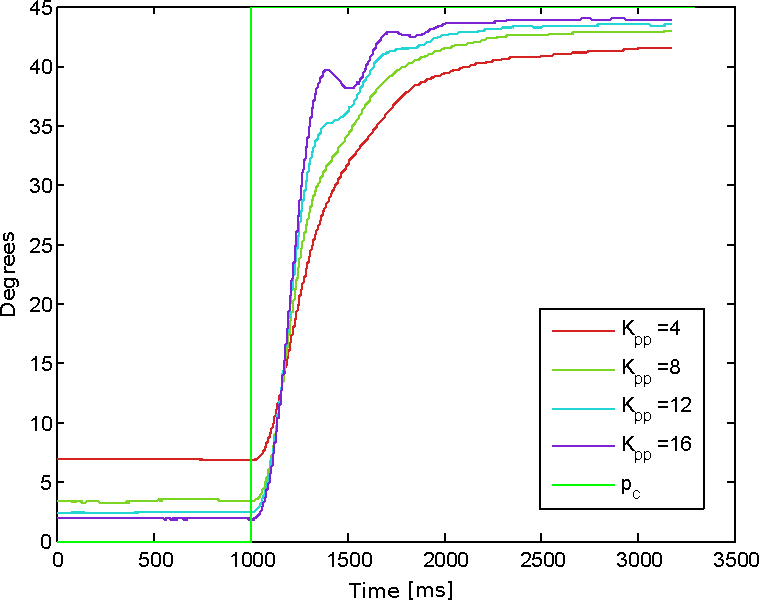
\includegraphics[width=1\textwidth,trim={0cm 0cm 0cm 0cm},clip]{figures/P2p1_K_pp_label.pdf}
	\caption{Pitch response with PD control}
\label{fig:P2p1_K_pp}
\end{figure}
\begin{figure}[!!ht!!!!!!!!tb!!]
	\centering
		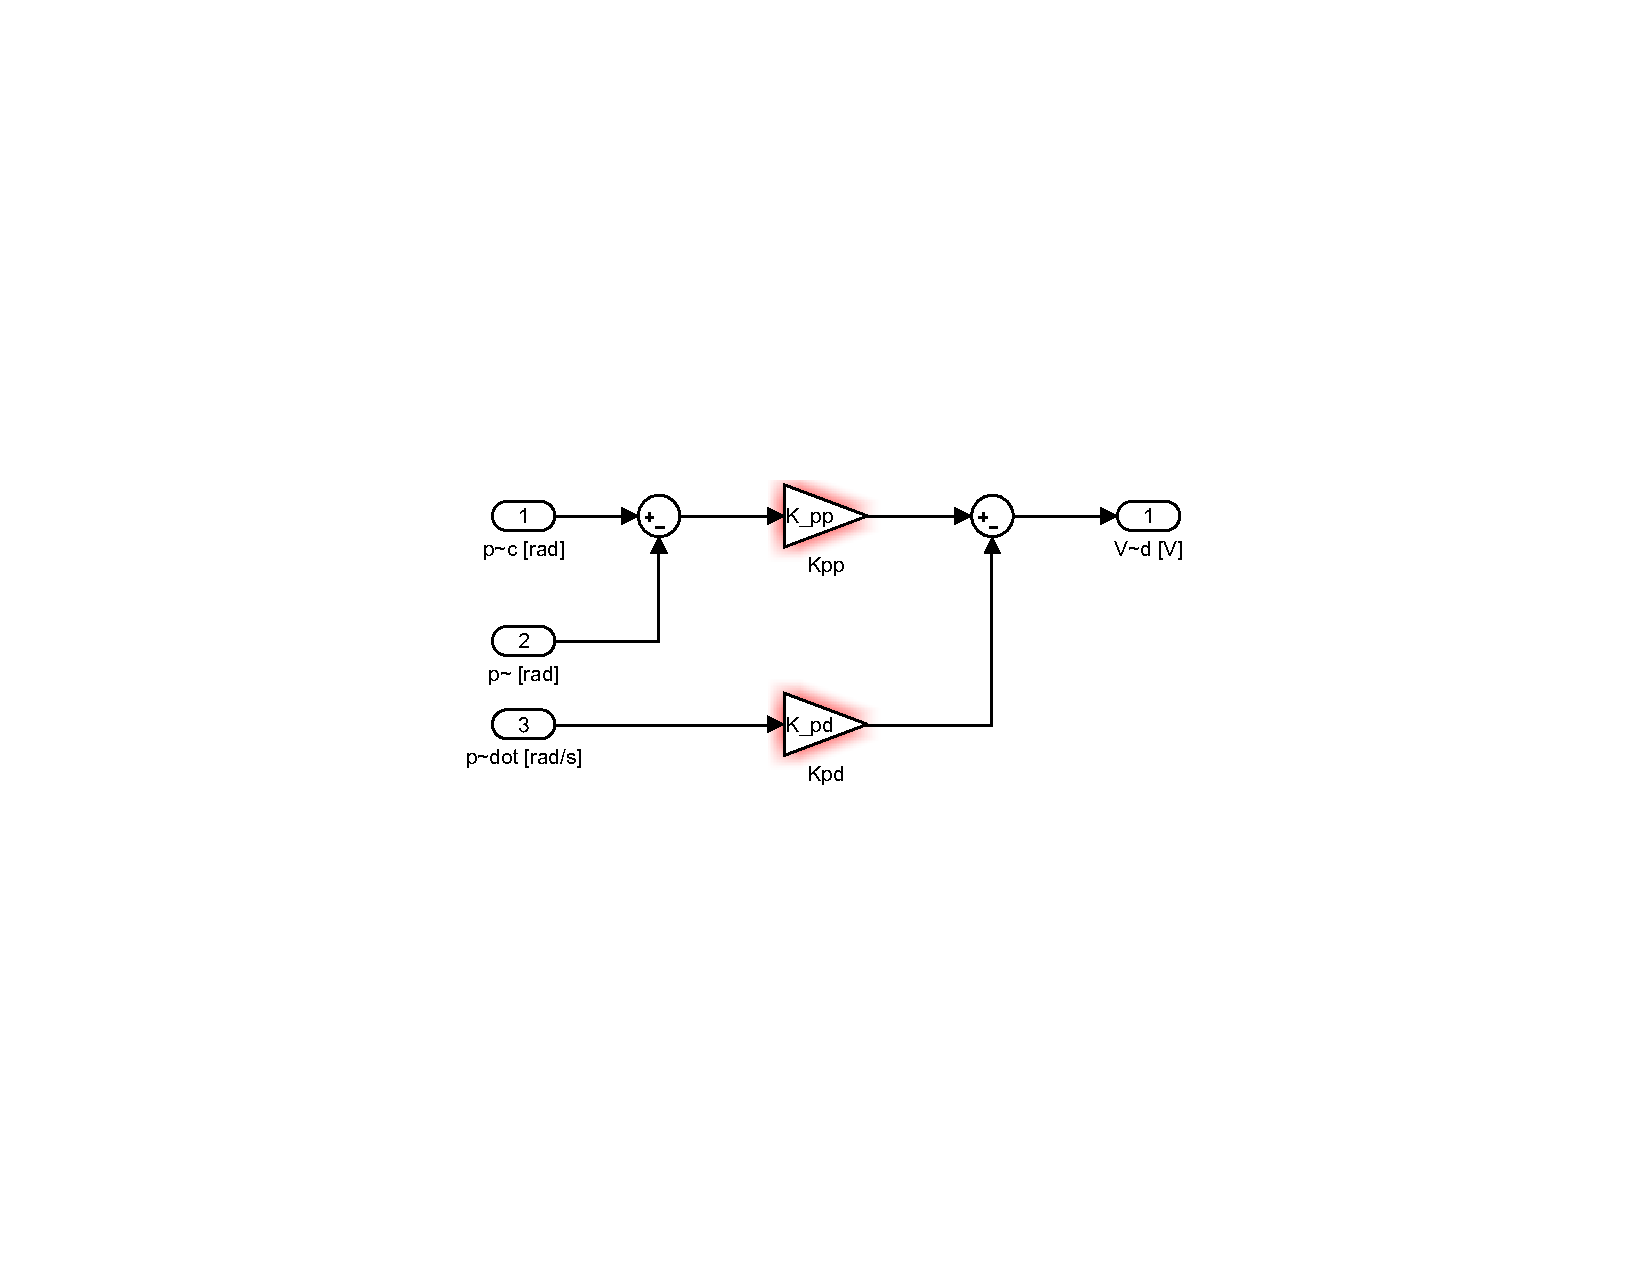
\includegraphics[scale=0.9, trim={6.2cm 8cm 0cm 4cm},clip]{figures/simulink/PD_controller.pdf}
	\caption{Inside the Pitch controller}
\label{fig:P2p1_controller}
\end{figure}
\clearpage
